\section{Results}
\label{sec:results}

In this section we present the main results of this work, namely the determination
of the photon PDF $\gamma(x,Q^2)$ from a fit to the HERA structure functions
and ATLAS high-mass Drell-Yan cross-sections.

Using the NNLO fit settings discussed in Sect.~\ref{sec:fitsettings}, we find
a $\chi^{2}/N_{\rm dof} = 1.18$,
with a partial $\chi^2/N_{\rm dof} = 1.15$ for the high-mass Drell-yan data.
%
First of all we present our results for the photon PDF, and then the impact
of the DY measurements on the quark and gluon PDF.
%
In Fig.~\ref{photon_zoom} we show our results
for $\gamma(x,Q^2)$ for $Q^2=10^4$ GeV$^2$,
compared with LUXqed~\cite{Manohar:2016nzj}, HKR~\cite{Harland-Lang:2016apc}
and NNPDF3.0QED.
%
The comparison is restricted to the range $0.05 \le x \le 0.3$ corresponding
to the region where the fitted Drell-Yan measurements have direct kinematic sensitivity
to the photon PDF.
%
For NNPDF3.0QED, we show the 68\% CL uncertainty, while for LUXqed the uncertainty band
is obtained by adding in quadrature all the model variations.

%%%%%%%%%%%%%%%%%%%%%%%%%%%%%%%%%%%%%%%%%%%%%%%%%%%%%%%%
\begin{figure}[h]
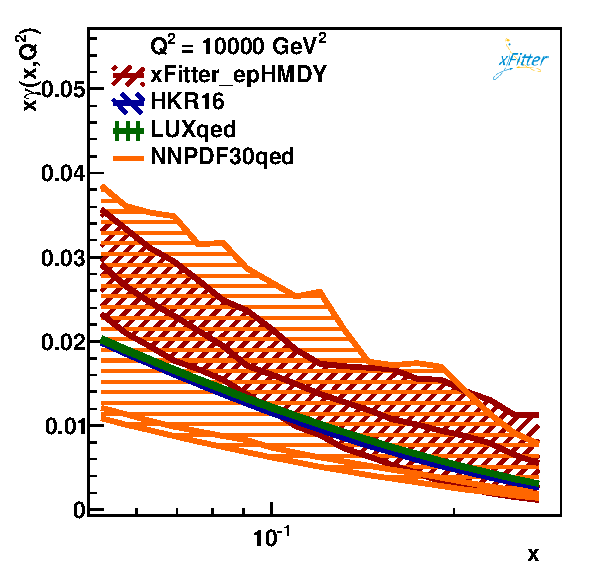
\includegraphics[width=7cm]{plots/photon_comp_10000.pdf} 
\caption{Comparison between $\gamma(x,Q^2)$ at $Q^2=10^4$ GeV$^2$ in the present
  analysis with the corresponding results from NNPDF3.0QED, LUXqed and HKR.}
\label{photon_zoom}
\end{figure}
%%%%%%%%%%%%%%%%%%%%%%%%%%%%%%%%%%%%%%%%%%%%%%%%%%%%%%%%

From the results of Fig.~\ref{photon_zoom} we find that in the region where the HMDY data is
sensitive to the photon PDF, there is good agreement between the four determinations.
%
As compared to NNPDF3.0QED, the PDF uncertainties in the current analysis are reduced, though
they are still not competitive with those of LUXqed.
%
We also note the excellent agreement between the LUXqed and the HKN determinations.

We now turn the comparison to the quark and gluon PDFs.
%
Here we will compare a reference fit with the same settings as in Sect.~\ref{sec:fitsettings}
but with only the HERA inclusive structure function data with the results of this work,
which also include the ATLAS high-mass DY measurements.
%
We do not attempt to compare as well with the global fits, since our motivation here is only to
gauge the impact on quarks and gluons of the high-mass Drell-Yan data.

Fig.~\ref{PDF_7.5GeV}
 shows the PDF distributions $x_{u_v},xd_{d_v},x\bar{u}, x\bar{d}, xg$ at $Q^{2}$ = 7.5$^{2}$ GeV$^{2}$,
including model and parametrisation uncertainties, while  Fig.~\ref{PDF_10000GeV} 
shows them at $Q^{2}$ = 10$^{4}$ GeV$^{2}$. {\it Add model and parametrisation variations, Use NNLO MC central}.
\begin{figure}
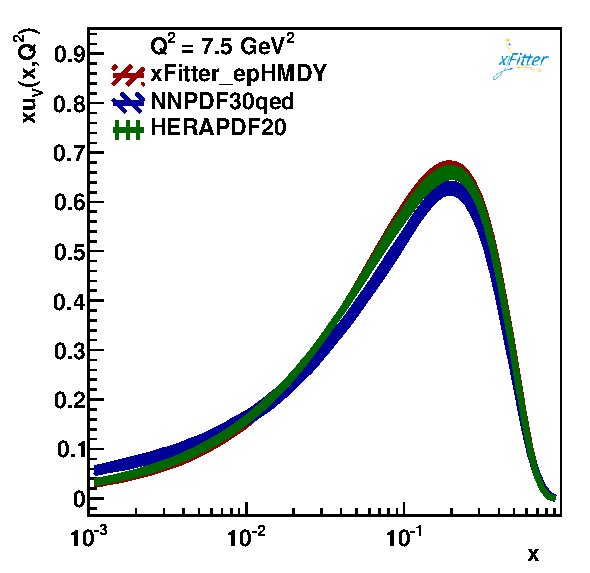
\includegraphics[width=7cm]{plots/uv_7_5.pdf} 
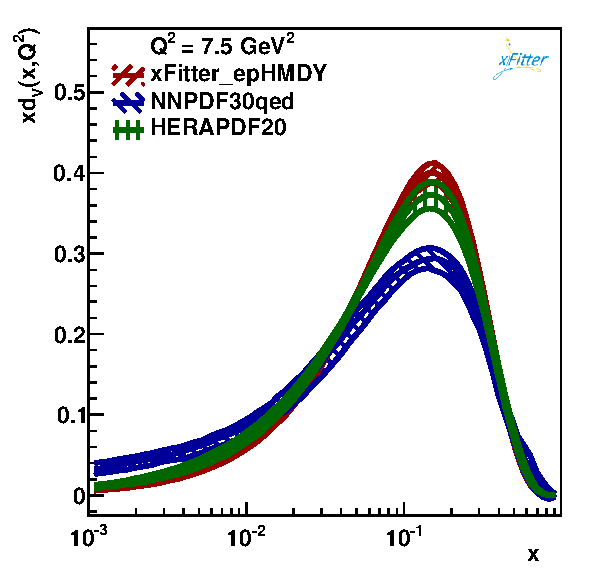
\includegraphics[width=7cm]{plots/dv_7_5.pdf} 
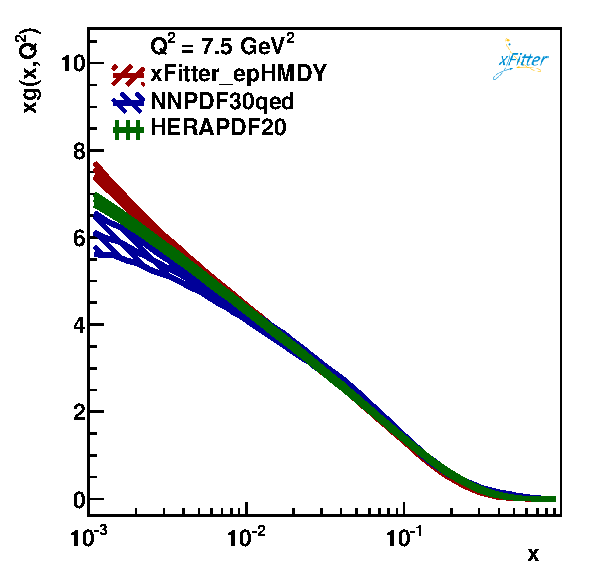
\includegraphics[width=7cm]{plots/gluon_7_5.pdf} 
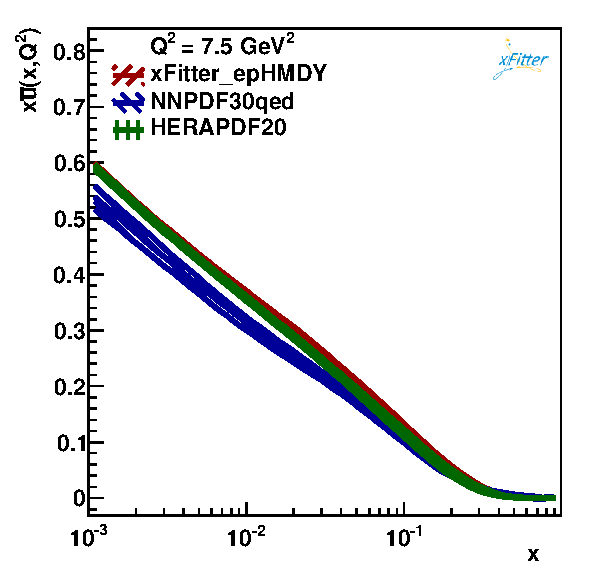
\includegraphics[width=7cm]{plots/ubar_7_5.pdf} 
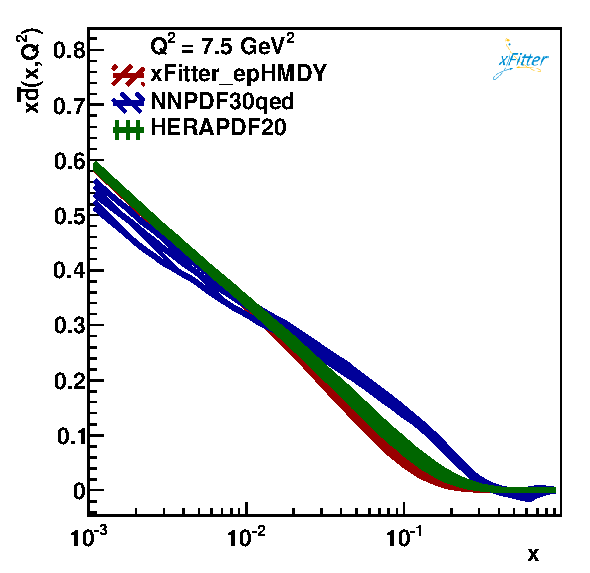
\includegraphics[width=7cm]{plots/dbar_7_5.pdf} 
\caption{NNLO PDF distributions at $Q^{2}$ = 7.5$^{2}$ GeV$^{2}$: (a) $u$ - valence; (b) $d$ - valence; (c) gluon; (d) $\bar{u}$; (e) $\bar{d}$ }
\label{PDF_7.5GeV}
\end{figure}
\begin{figure}
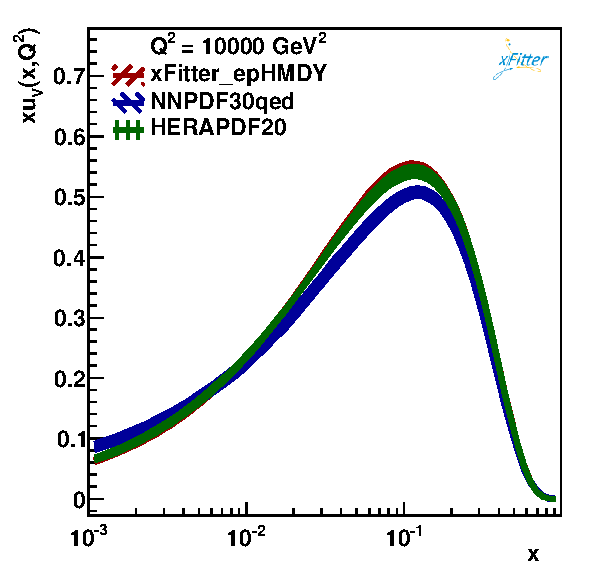
\includegraphics[width=7cm]{plots/uv_10000.pdf} 
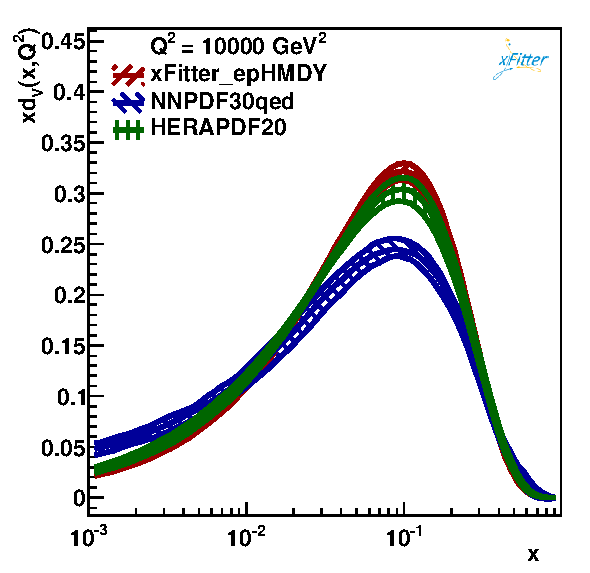
\includegraphics[width=7cm]{plots/dv_10000.pdf} 
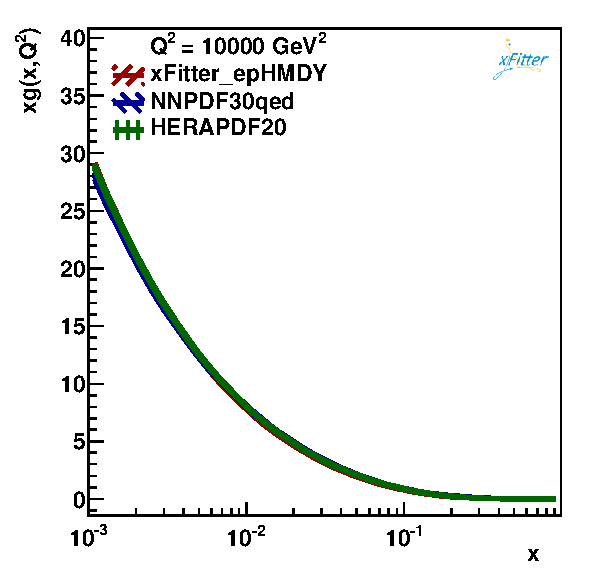
\includegraphics[width=7cm]{plots/gluon_10000.pdf} 
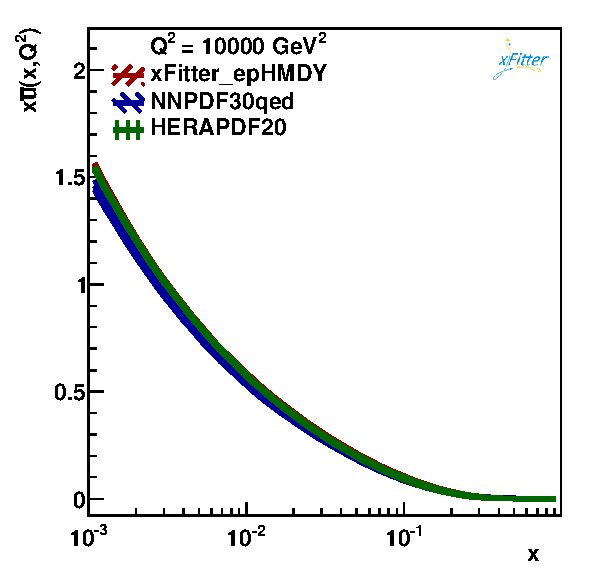
\includegraphics[width=7cm]{plots/ubar_10000.pdf} 
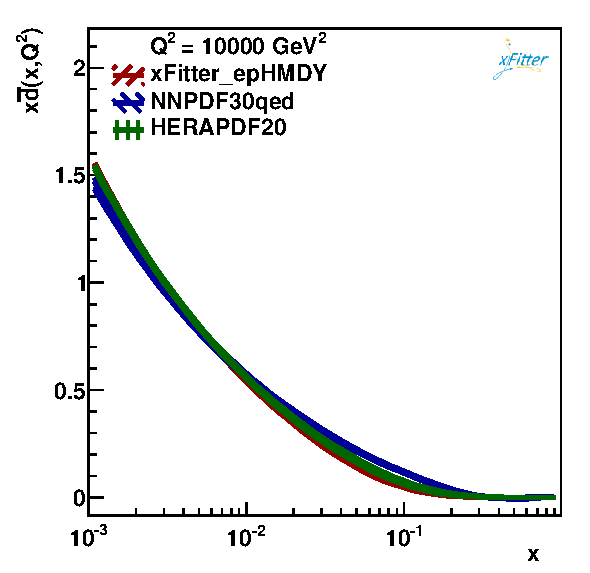
\includegraphics[width=7cm]{plots/dbar_10000.pdf} 
\caption{NNLO PDF distributions at $Q^{2}$ = 10000$^{2}$ GeV$^{2}$: (a) $u$ - valence; (b) $d$ - valence; (c) gluon; (d) $\bar{u}$; (e) $\bar{d}$}
\label{PDF_10000GeV}
\end{figure}
In these figures comparisons are made to the NNPDF3.0PDF set and the HERAPDF2.0 set.
The shape of the $xd_{u_v}$ distribution is close to that of HERAPDF2.0 
because of the dominance of HERA data in the fit. 


Fig.~\ref{hmDY_2D} 
shows the comparison between the high-mass Drell-Yan double differential distribution and 
the predictions.
\begin{figure}
\centering
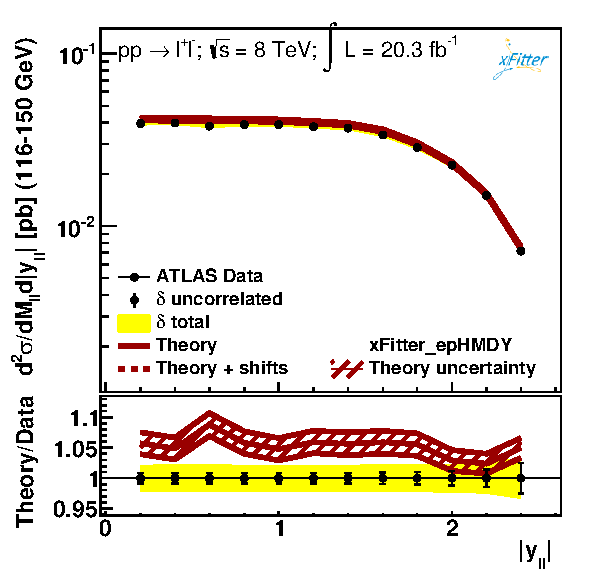
\includegraphics[width=7cm]{plots/data_1.pdf} 
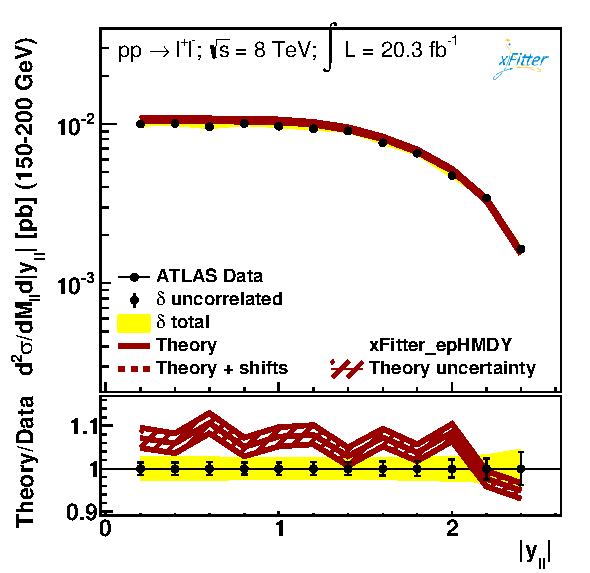
\includegraphics[width=7cm]{plots/data_2.pdf} 
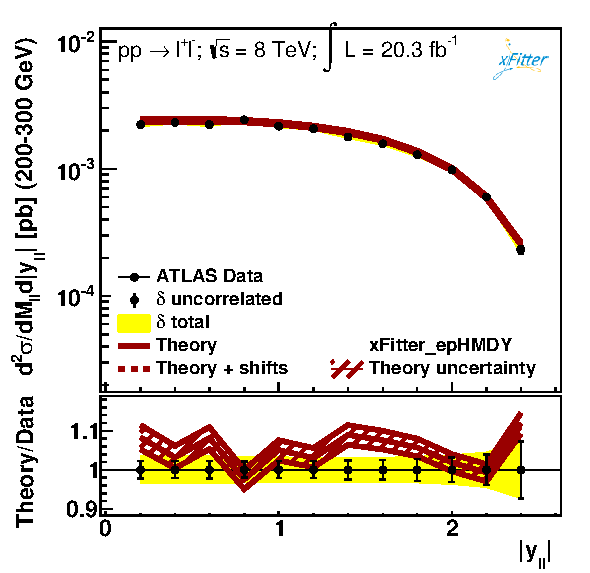
\includegraphics[width=7cm]{plots/data_3.pdf} 
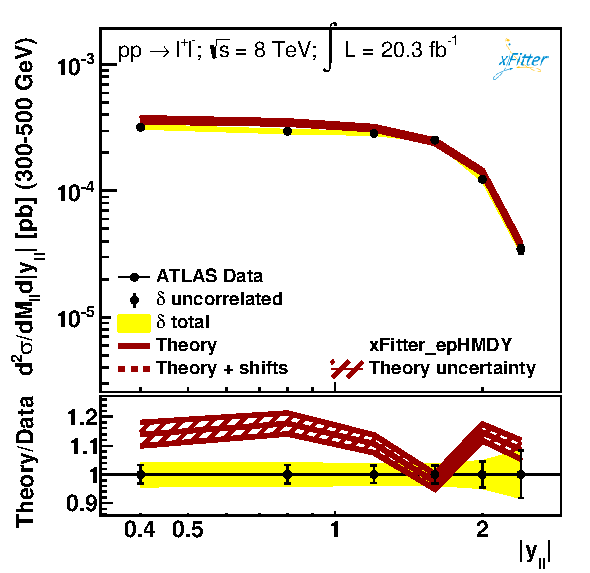
\includegraphics[width=7cm]{plots/data_4.pdf} 
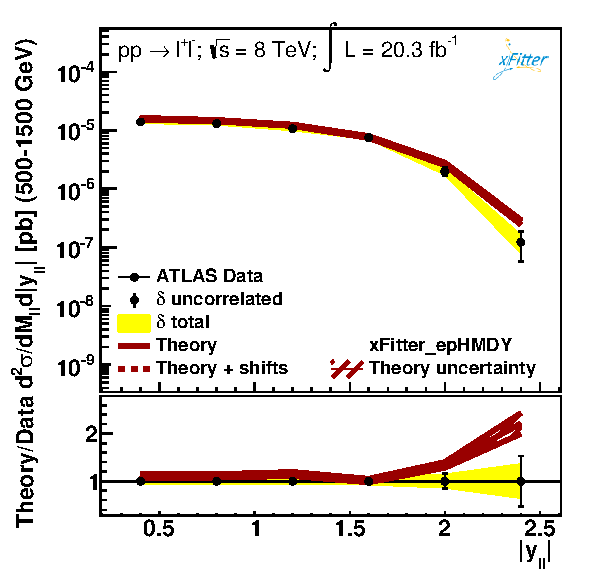
\includegraphics[width=7cm]{plots/data_5.pdf} 
\caption{Comparison between $\frac{d^{2}\sigma}{dm_{ll}d|y_{ll}|}$ for the high-mass Drell Yan data and the NNLO fit predictions.}
\label{hmDY_2D}
\end{figure}
The $\chi^{2}$ values for the high-mass Drell Yan data and the output parameters from NNLO fit can be found in Table.~\ref{chi2_scan} 
and Table.~\ref{par_scan} 
respectively. 
\begin{figure}
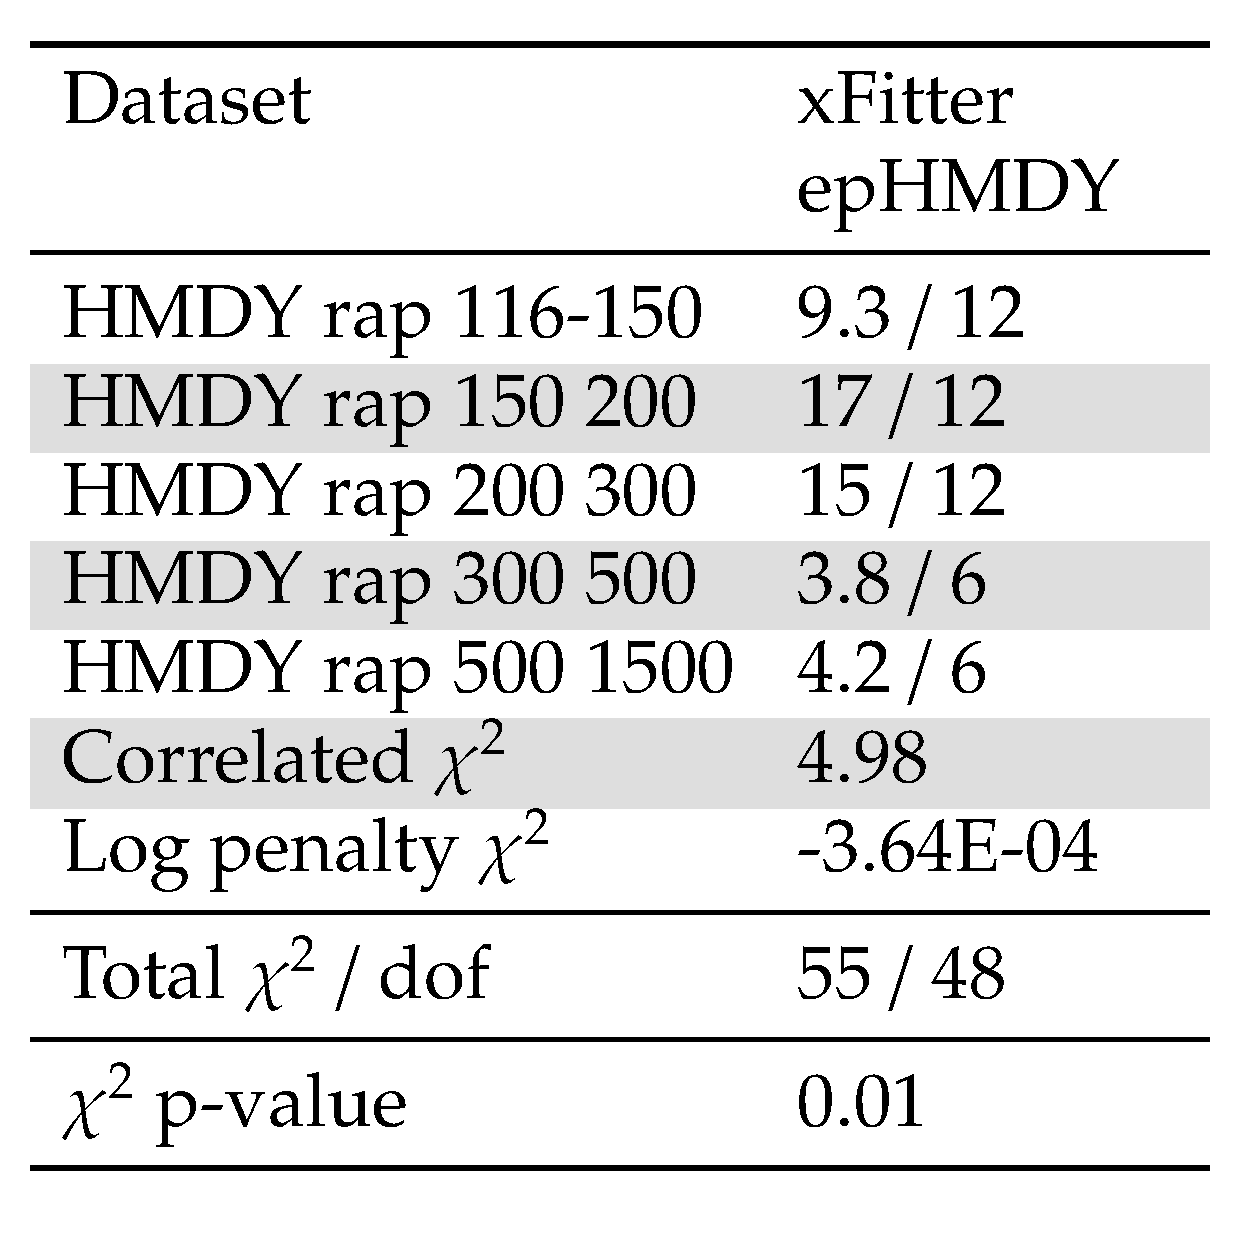
\includegraphics[width=14cm]{plots/chi2_hmDY.pdf} 
\caption{$\chi^{2}$ for high-mass Drell Yan data, for the NNLO fit}
\label{chi2_scan}
\end{figure}
\begin{figure}
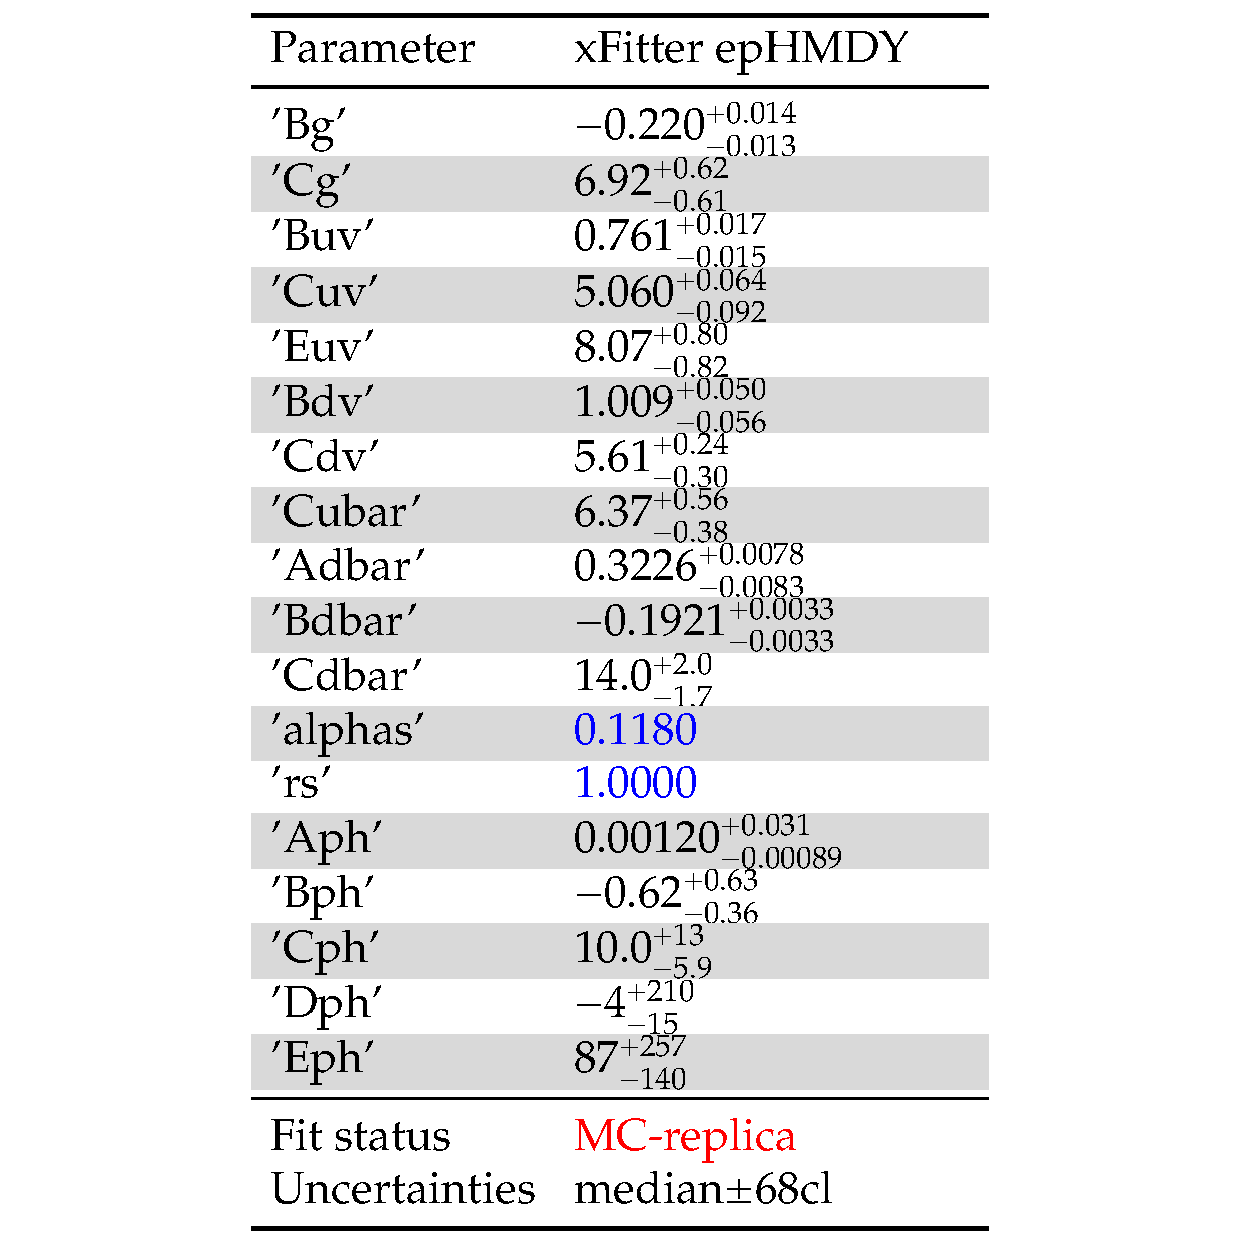
\includegraphics[width=14cm]{plots/parameters.pdf} 
\caption{PDF parameters for the NNLO fit.}
\label{par_scan}
\end{figure}

The NNLO photon PDF distribution is shown 
both at the starting scale (7.5 GeV$^{2}$) and at 10$^{4}$ GeV$^{2}$ 
 in Fig.~\ref{photon}, where it is also compared to an NLO extraction of the photon distribution.
The $x$-range of the figure is restricted to the range of sensitivity of the high-mass Drell-Yan data;
$0.045 < x < 0.35$. The NLO and NNLO photon PDFs are compatible over this range.
\begin{figure}
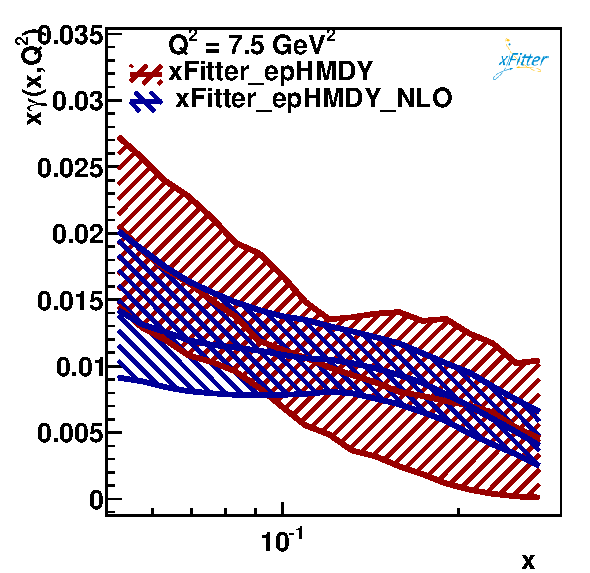
\includegraphics[width=7cm]{plots/photon_7_5.pdf} 
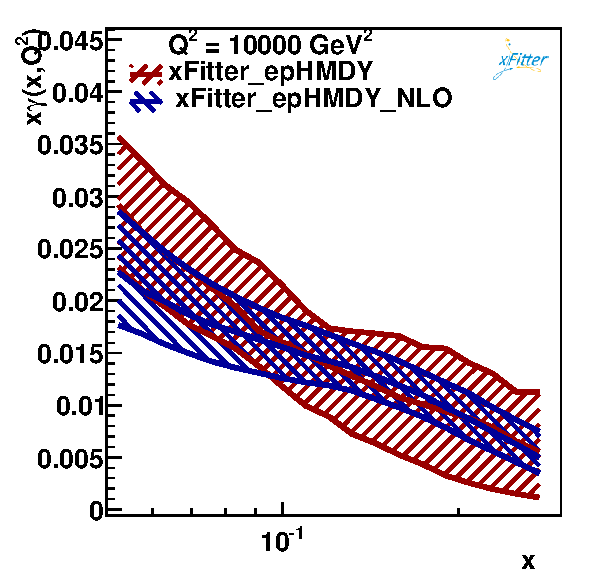
\includegraphics[width=7cm]{plots/photon_10000.pdf} 
\caption{Comparison between the photon PDF distributions at NNLO and NLO: (a) at the starting scale; (b) at the evolved scale.}
\label{photon}
\end{figure}


Comparison with the data
